\documentclass[11pt]{article}
\usepackage{amsmath, amssymb, amsthm}
\usepackage{graphicx}
\usepackage{float}

\begin{document}

\section*{Problem 1 --- Linear Regression / SVD}

\noindent\textbf{(a)} The empirical squared-loss risk is
\begin{align*}
\hat R(w) &= \frac{1}{2n}\sum_{i=1}^d \sum_{j=1}^{n_i} (w_i - y_{ij})^2.
\end{align*}
Differentiating coordinate-wise and setting to zero gives
\begin{align*}
w_i = \frac{1}{n_i}\sum_{j=1}^{n_i} y_{ij}.
\end{align*}

\noindent\textbf{(b)} With $X = \sum_{t=1}^r s_t u_t v_t^\top$ and $y \in \text{span}\{u_1,\dots,u_r\}$, let
\begin{align*}
w = \sum_{t=1}^r \frac{\beta_t}{s_t} v_t, \qquad \text{where } y = \sum_{t=1}^r \beta_t u_t.
\end{align*}
Then
\begin{align*}
Xw = y,
\end{align*}
so the empirical risk is zero.
\vspace{1em} 
\newline
\noindent\textbf{(c)} The nonzero eigenvalues of $X^\top X$ are $s_1^2,\dots,s_r^2$.  
If the rows of $X$ span $\mathbb{R}^d$, then $\text{rank}(X)=d$ and $X^\top X$ is invertible.  
Conversely, if $X^\top X$ is invertible, then $\text{rank}(X)=d$, hence the rows span $\mathbb{R}^d$.

\vspace{1em} 

\noindent\textbf{(d)} Example:
\begin{align*}
X &= \begin{pmatrix} 1 & 0 \\ 0 & 1 \\ 0 & 0 \end{pmatrix}, \qquad
X^\top X = I_2 \ \text{(invertible)}, \qquad
XX^\top = \begin{pmatrix} 1 & 0 & 0 \\ 0 & 1 & 0 \\ 0 & 0 & 0 \end{pmatrix} \ \text{(not invertible)}.
\end{align*}

\section*{Problem 2 --- Linear Regression}

\noindent\textbf{(a), (b)} \quad [skiped: code]
\noindent\textbf{(c)} 

\begin{figure}[H]
  \centering
  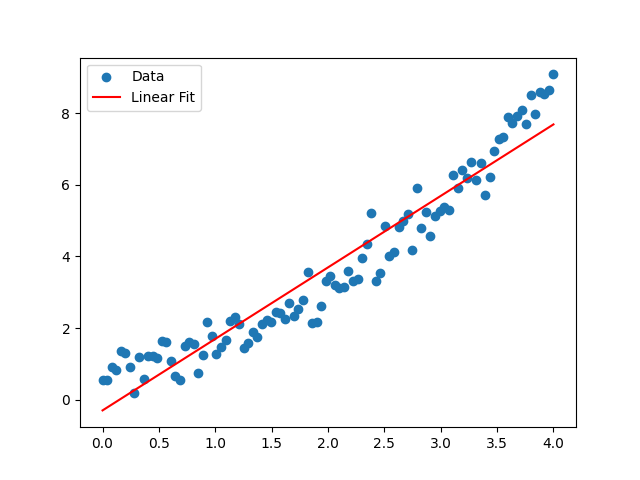
\includegraphics[width=0.7\linewidth]{2-c-output.png}
  \caption{Linear fit and data (Problem 2(c))}
  \label{fig:2c-linear-fit}
\end{figure}

\section*{Problem 3 --- Polynomial Regression}

\noindent\textbf{(a)} For $x=(x_1,x_2,x_3)$,
\begin{align*}
\phi(x) = \big[1,\; x_1,\; x_2,\; x_3,\; x_1^2,\; x_1x_2,\; x_1x_3,\; x_2^2,\; x_2x_3,\; x_3^2\big]^\top.
\end{align*}

\noindent\textbf{(b) to (e)} \quad [skiped: code]

\noindent\textbf{(d)} 
\begin{figure}[H]
  \centering
  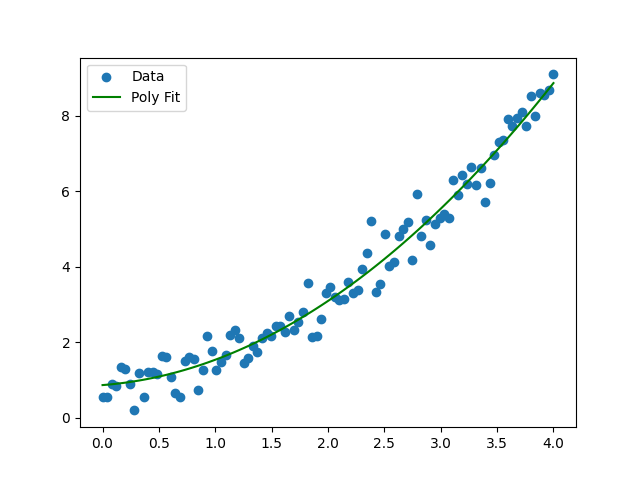
\includegraphics[width=0.7\linewidth]{3-d-output.png}
  \caption{Polynomial fit and data (Problem 3(d))}
  \label{fig:3d-poly-fit}
\end{figure}

The polynomial model (quadratic expansion) appears to approximate the data better than the linear model from Problem 2. The quadratic fit follows the curvature present in the data (the generating process includes an $x^2$ term), reducing systematic bias seen in the linear fit. In contrast, the linear model cannot capture the curvature and yields larger residuals particularly where the true function bends.

\noindent\textbf{(e)} 

\begin{figure}[H]
  \centering
  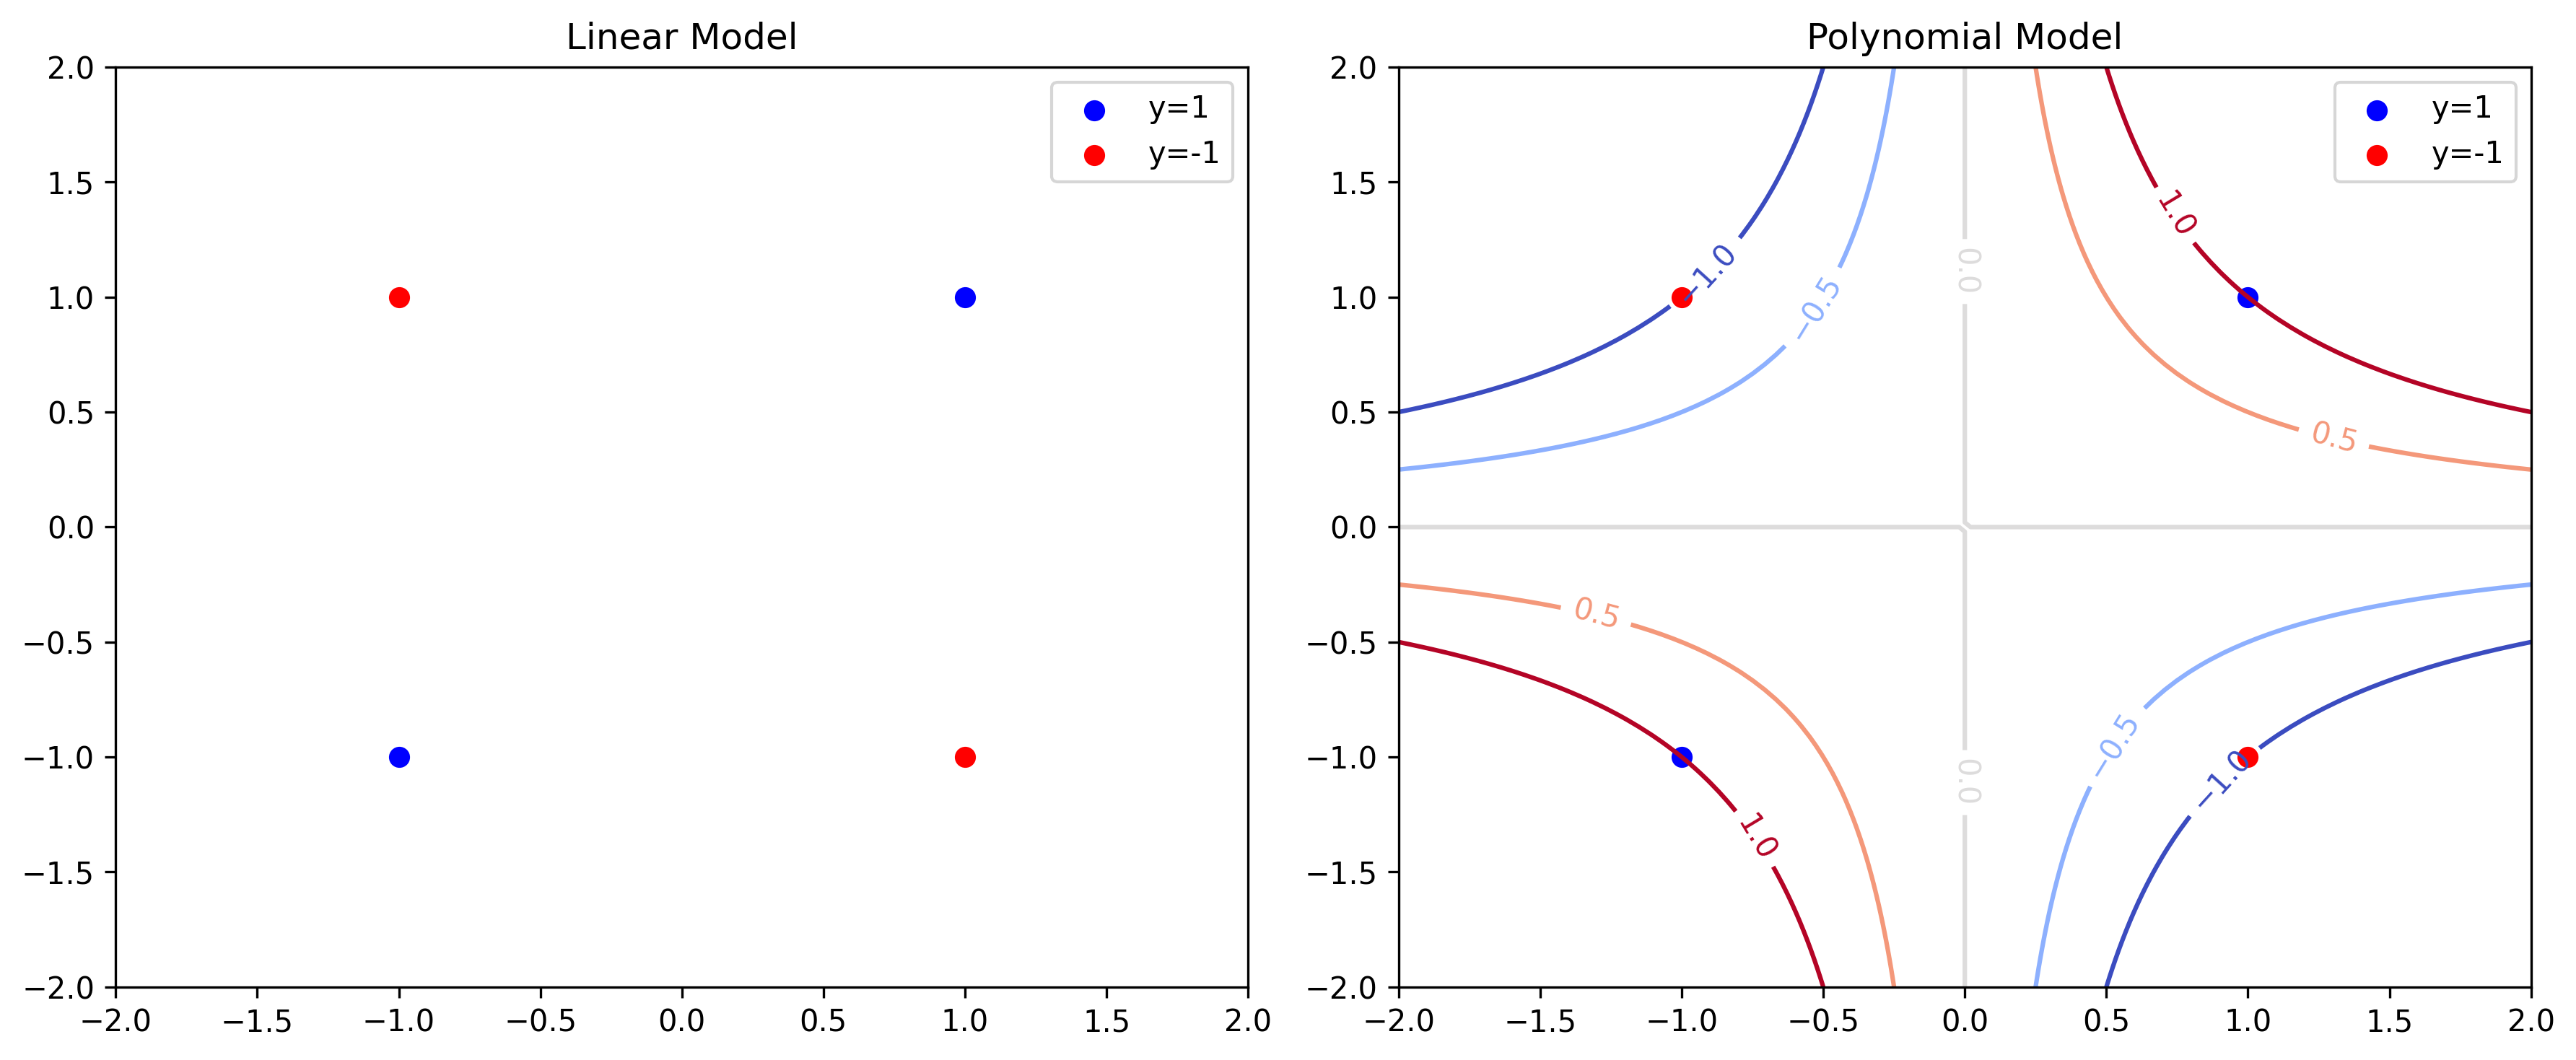
\includegraphics[width=0.9\linewidth]{3-e-output.png}
  \caption{XOR Classification with Linear and Polynomial Models}
  \label{fig:xor-classification}
\end{figure}

For the XOR classification problem, the linear model fails to correctly classify all points because XOR is not linearly separable. The decision boundary (shown by the contour at level 0) in the linear model cannot separate the points with different labels. In contrast, the polynomial model with quadratic features can successfully classify all points by creating a more complex decision boundary that properly separates the positive and negative examples. This demonstrates why polynomial features are necessary for the XOR problem.

\section*{Problem 4 --- Logistic Regression}

\noindent\textbf{(a)} 
\begin{align*}
\hat R_{\log}(w) &= \frac1n \sum_{i=1}^n \ln\!\big(1+\exp(-y_i w^\top x_i)\big), \\
\nabla_w \hat R_{\log}(w) &= -\frac1n\sum_{i=1}^n y_i x_i\,\sigma(-y_i w^\top x_i), \\
w' &= w + \frac{\eta}{n}\sum_{i=1}^n y_i x_i\,\sigma(-y_i w^\top x_i).
\end{align*}

\noindent\textbf{(b), (c)}

\begin{figure}[H]
  \centering
  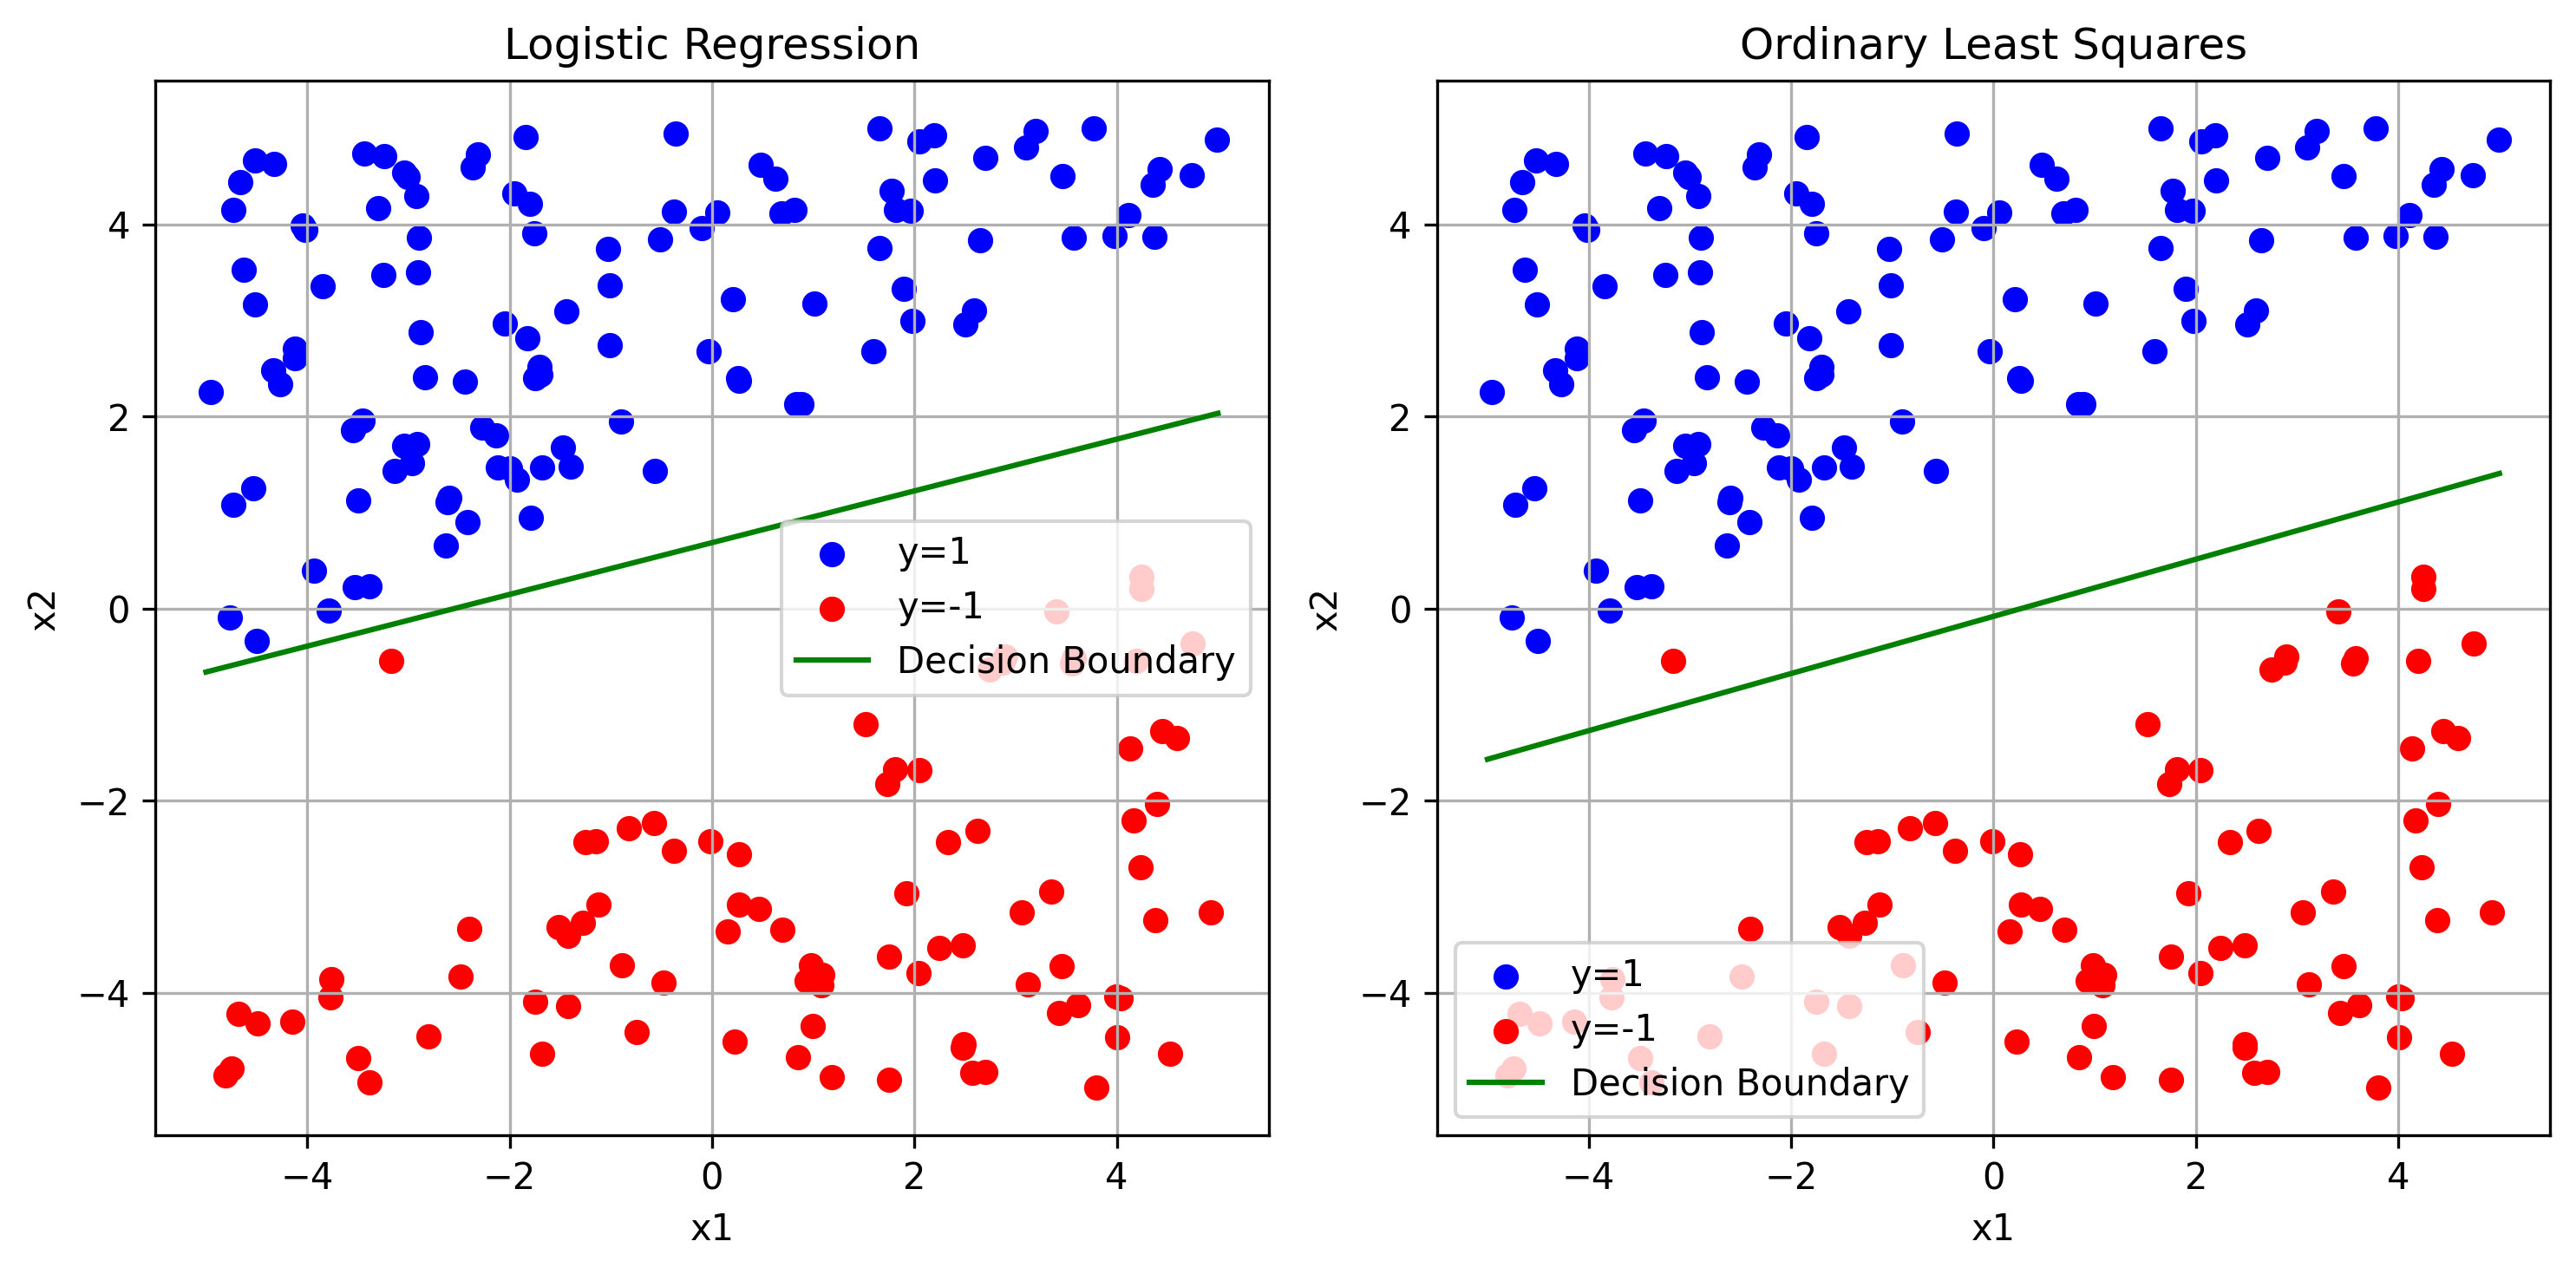
\includegraphics[width=0.9\linewidth]{4-c-output.png}
  \caption{Comparison of Logistic Regression and Ordinary Least Squares Classification}
  \label{fig:logistic-vs-ols}
\end{figure}

The logistic regression model appears to classify the data better than the ordinary least squares (OLS) model for several reasons:

1. The logistic regression model is specifically designed for classification tasks, as it directly optimizes the probability of correct classification through the logistic loss function.

2. The decision boundary found by logistic regression provides a clearer separation between the two classes, maintaining an appropriate margin from both classes.

3. The OLS model, while able to find a separating hyperplane, is less suitable for classification as it optimizes squared error loss, which doesn't directly correspond to classification accuracy and can be sensitive to the scale of the target values (-1 and 1).

4. The logistic regression's decision boundary is more robust because the logistic function saturates for points far from the boundary, making it less sensitive to outliers compared to the OLS model.

\section*{Problem 5 --- N-Gram Next Token Prediction (Cross-Entropy)}

\noindent\textbf{(a)} For sample $(x_i,y_i)$ with one-hot target $e_{y_i}$,
\begin{align*}
\nabla_W \ell_i(W) &= x_i\big(p(\cdot|x_i)-e_{y_i}\big)^\top, \\
\nabla_W \hat R_{\mathrm{CE}}(W) &= \frac1n \sum_{i=1}^n x_i\big(p(\cdot|x_i)-e_{y_i}\big)^\top, \\
W' &= W - \frac{\eta}{n} \sum_{i=1}^n x_i\big(p(\cdot|x_i)-e_{y_i}\big)^\top.
\end{align*}

\noindent\textbf{(b) to (d)} \quad [skipped: code]

\noindent\textbf{(e)} \quad Using the generate\_text() function ($n=4$, $embedding\_dim = 10$, $num\_tokens = 20$), here are five generated samples with different initial contexts:

\begin{itemize}
\item ``once upon a time in there magical rabbit there sky a wise howled owl...''
\item ``the wise old owl about hopped tales all crystal time colorful danced...''
\item ``deep in the crystal cave a dragon guarded ancient treasures and shared wisdom...''
\item ``under the starlit sky the wolves howled their ancient songs telling tales...''
\item ``by the enchanted lake fairies danced in circles spreading sparkles of magic...''
\end{itemize}

Two interesting patterns emerge: First, when the initial context exactly matches a training sequence (e.g., samples 3-5), the model generates coherent text for several tokens before degrading. Second, with unfamiliar contexts, the model immediately starts mixing unrelated story elements. This behavior stems from the n-gram model's limited context window ($n=4$): it can only maintain local word dependencies and lacks understanding of broader narrative structure.

\section*{Problem 6 --- LLM Use, Collaboration, and Other Sources}

\begin{enumerate}
\item GPT‘s assistant was used in Problems 1-5. Final answers were edited and revised manually. Then, used AI to reformat into Latex.
\item No additional external sources or collaborators were used.
\end{enumerate}

\end{document}
